\begin{frame}{Data --- Monte Carlo comparison (1)}
A comparison of the distribution of the relevant observables used in this
analysis was performed on real and simulated data, in order to assess the
reliability of Monte Carlo in computing efficiencies

\begin{center}
\scalebox{0.38}{
  \setlength{\unitlength}{1mm}
  \begin{picture}(150,140)
    %
    \put(0,0){
      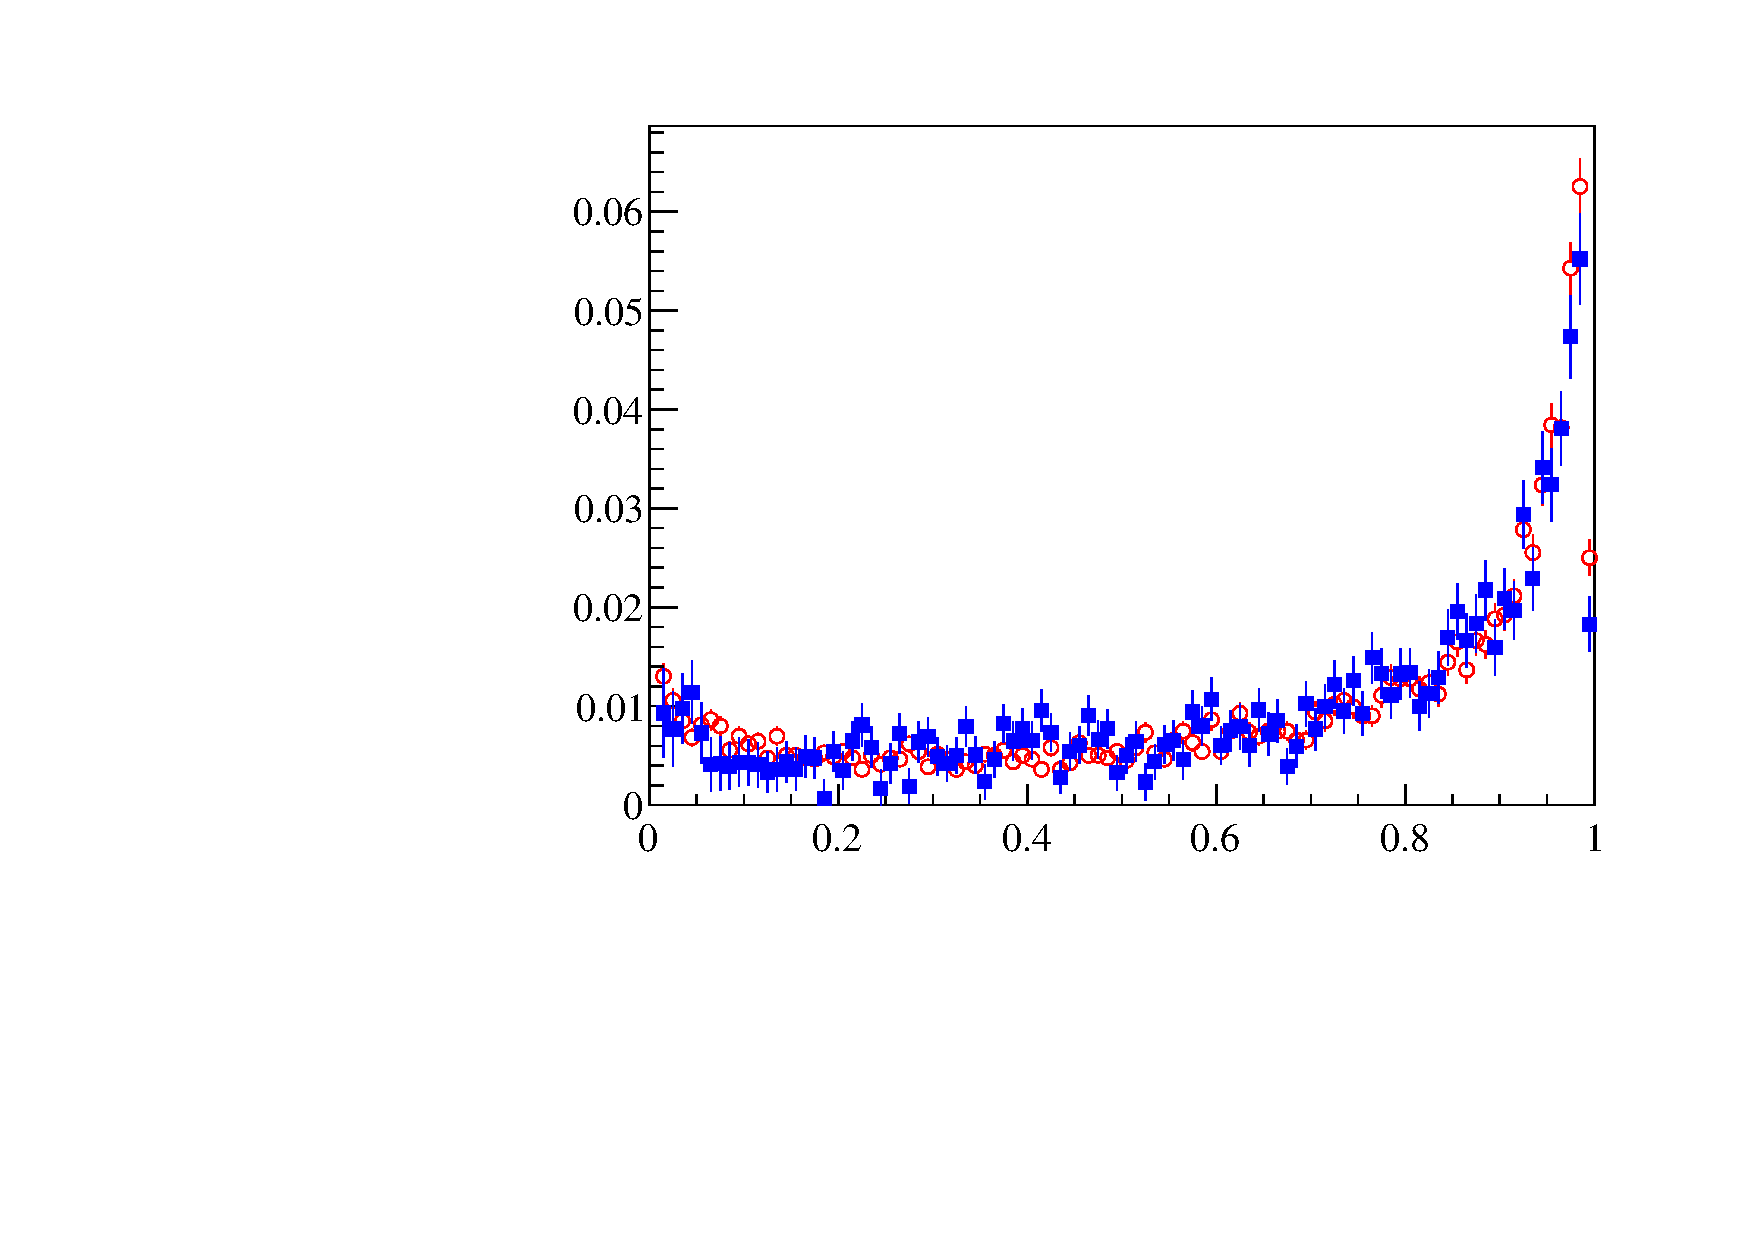
\includegraphics[width=50mm, height=35mm]{mc-data/cl_g_1p}
    }
    \put(50,0){
      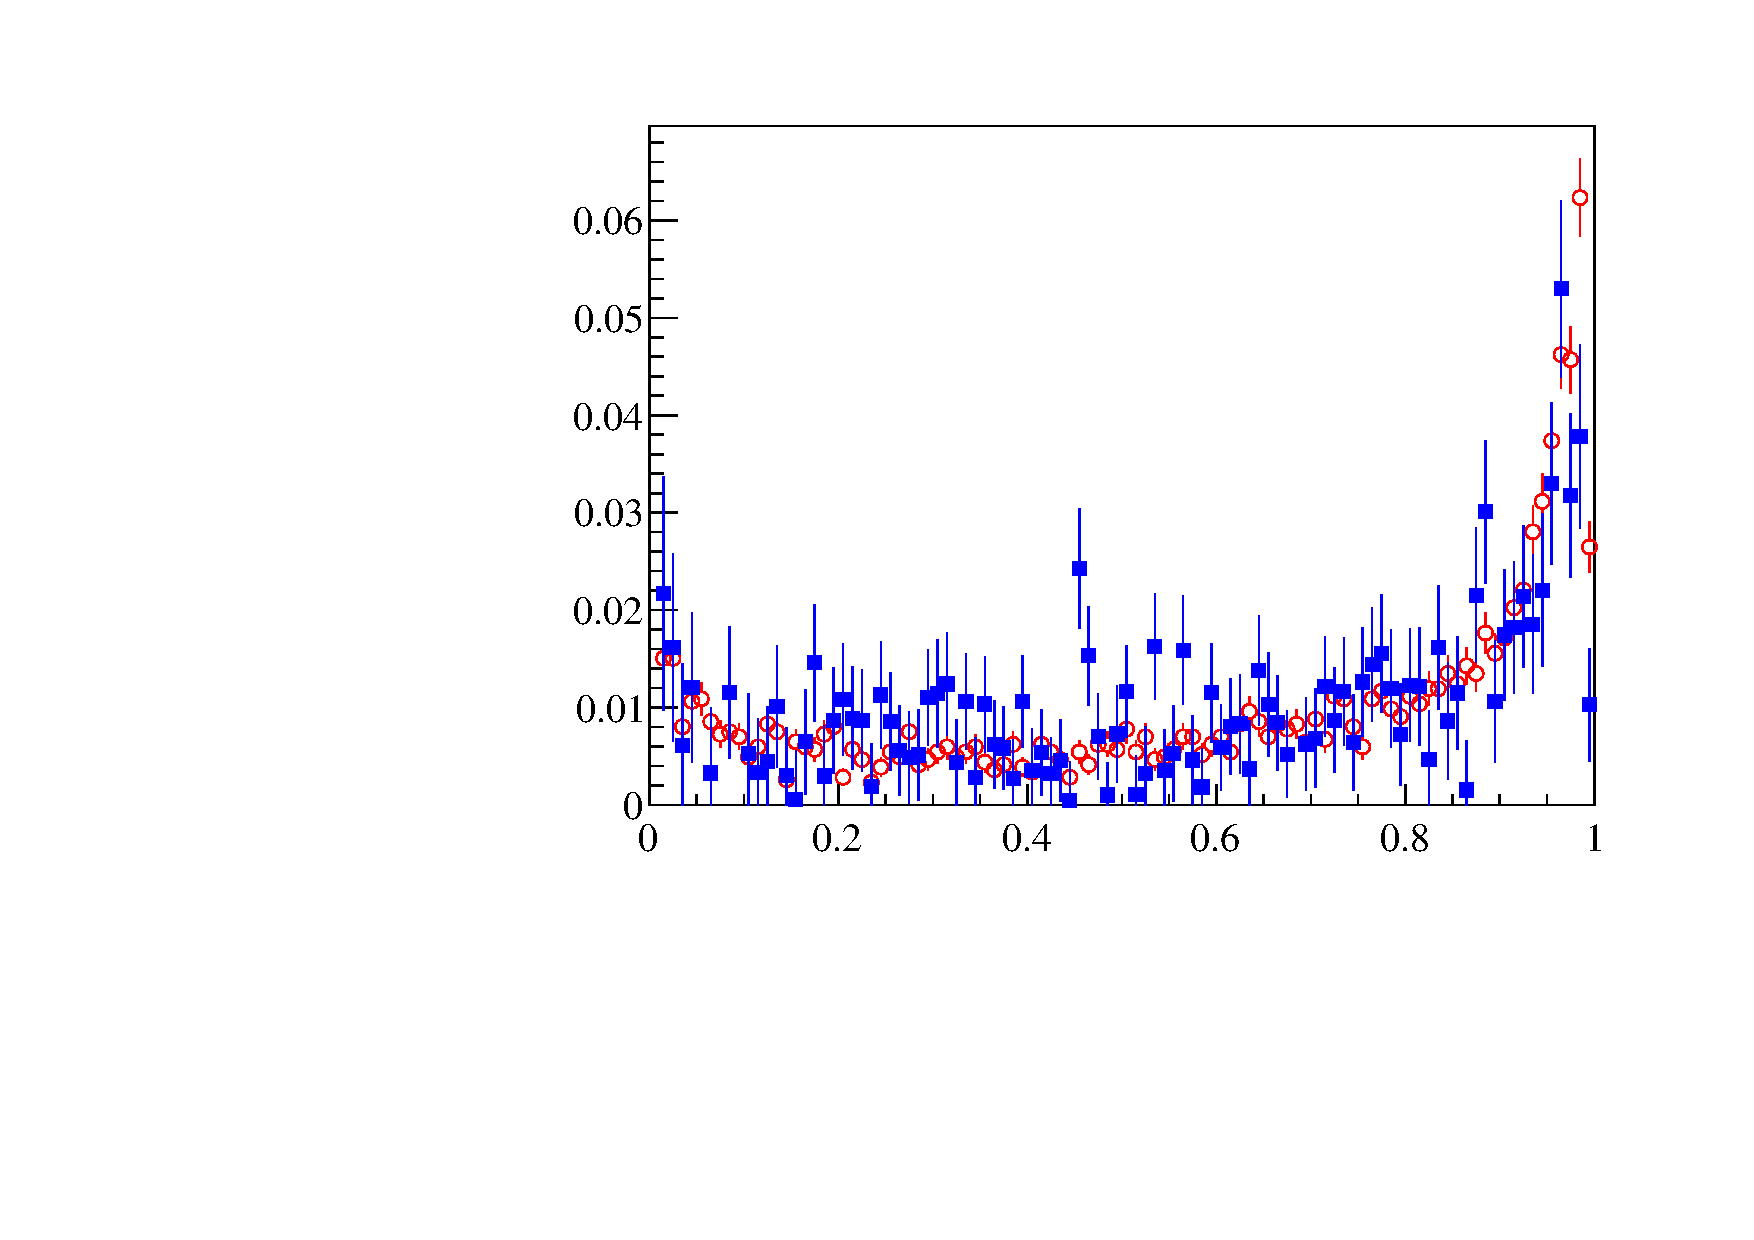
\includegraphics[width=50mm, height=35mm]{mc-data/cl_g_2p}
    }
    \put(100,0){
      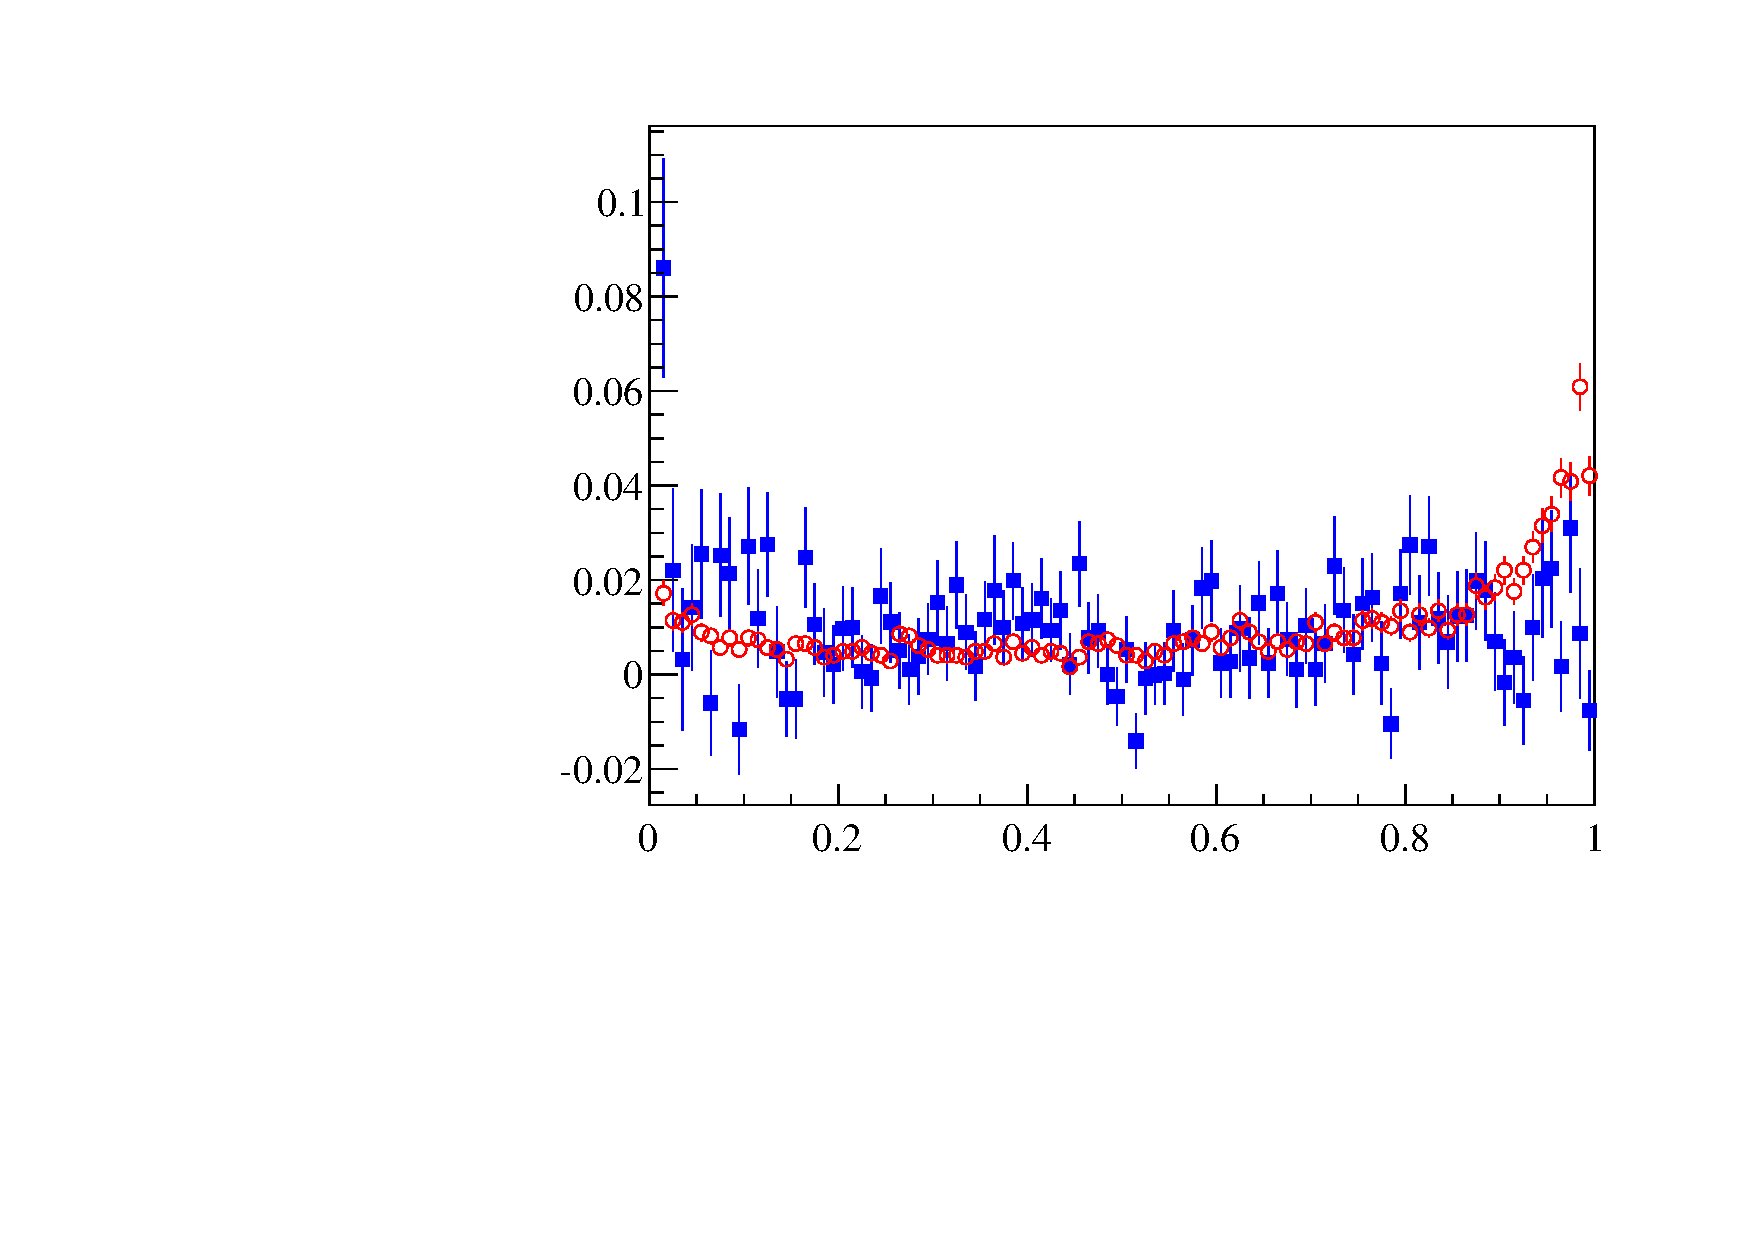
\includegraphics[width=50mm, height=35mm]{mc-data/cl_g_3p}
    }

    \put(0,35){
      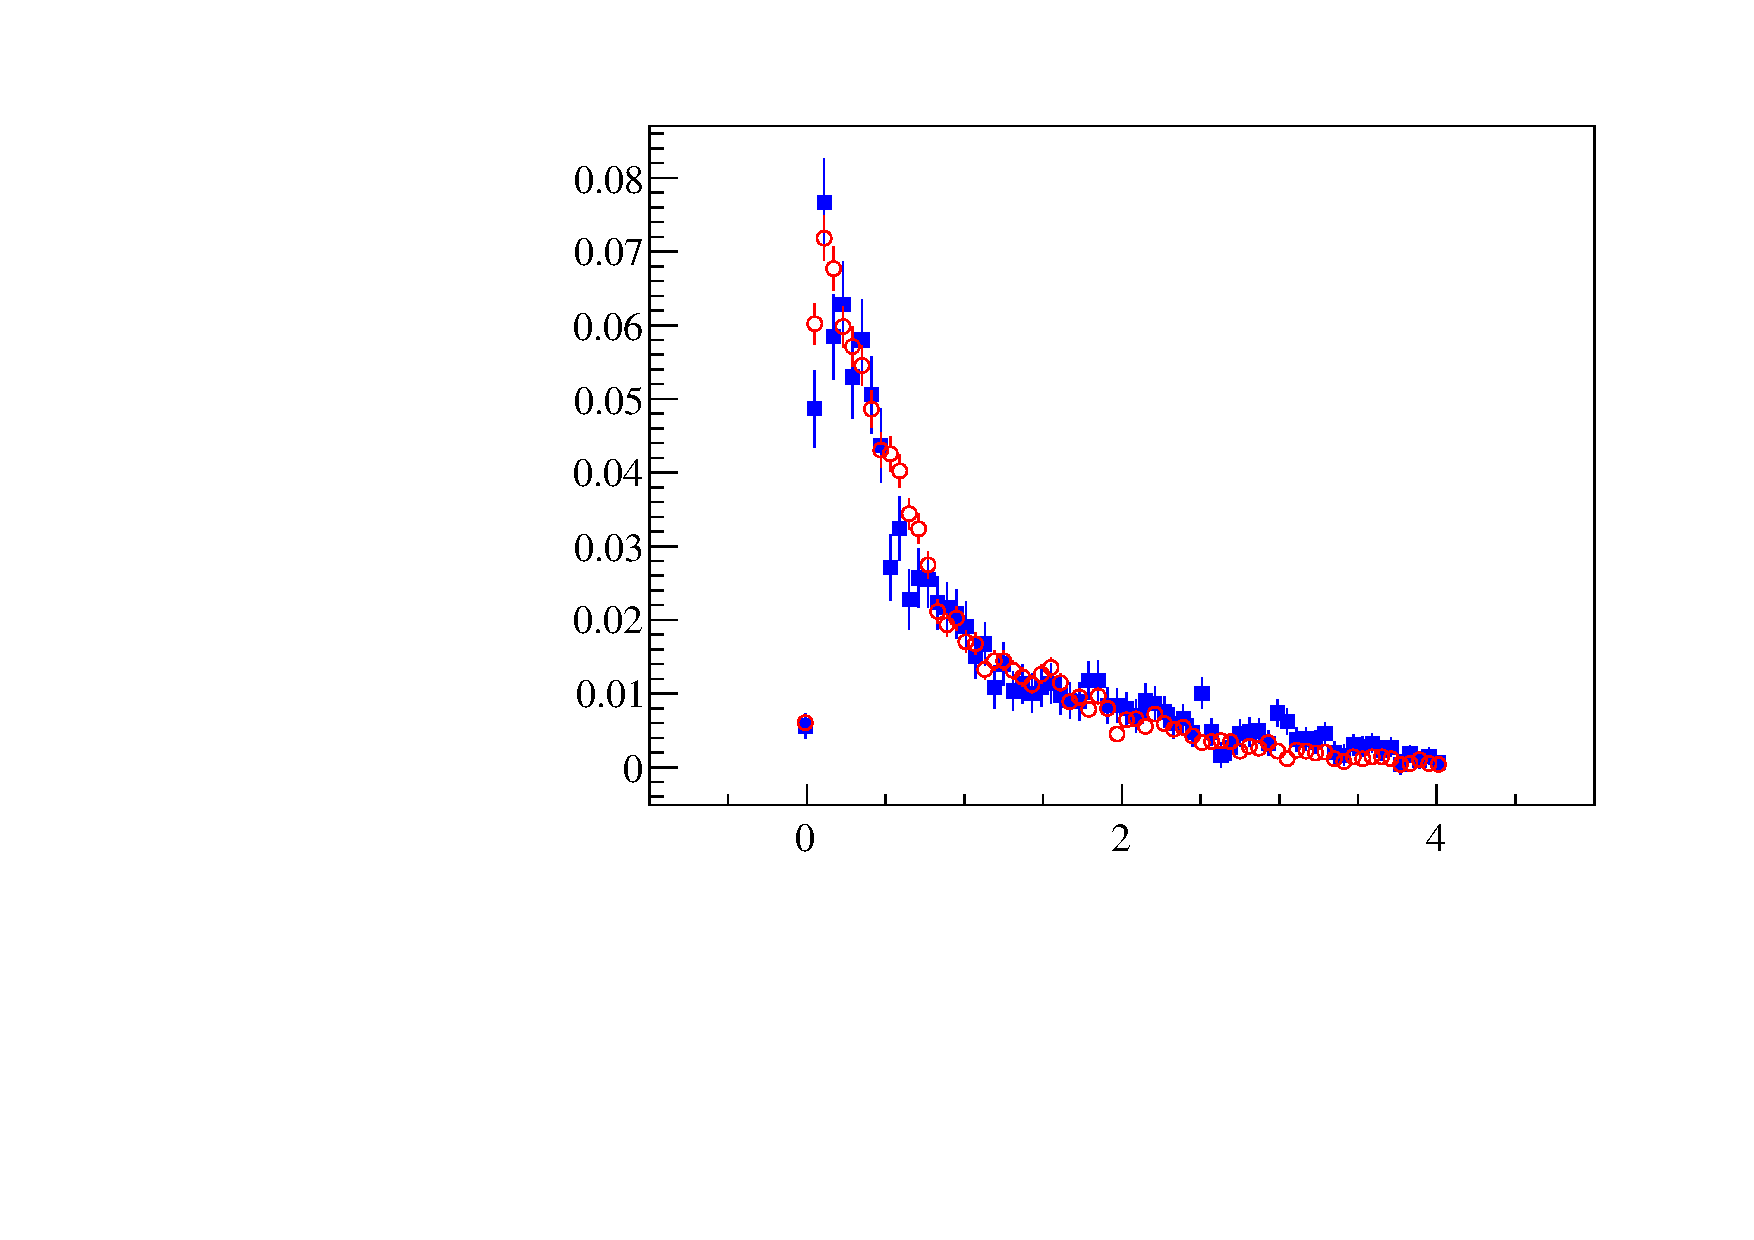
\includegraphics[width=50mm, height=35mm]{mc-data/c2_dtf_1p}
    }
    \put(50,35){
      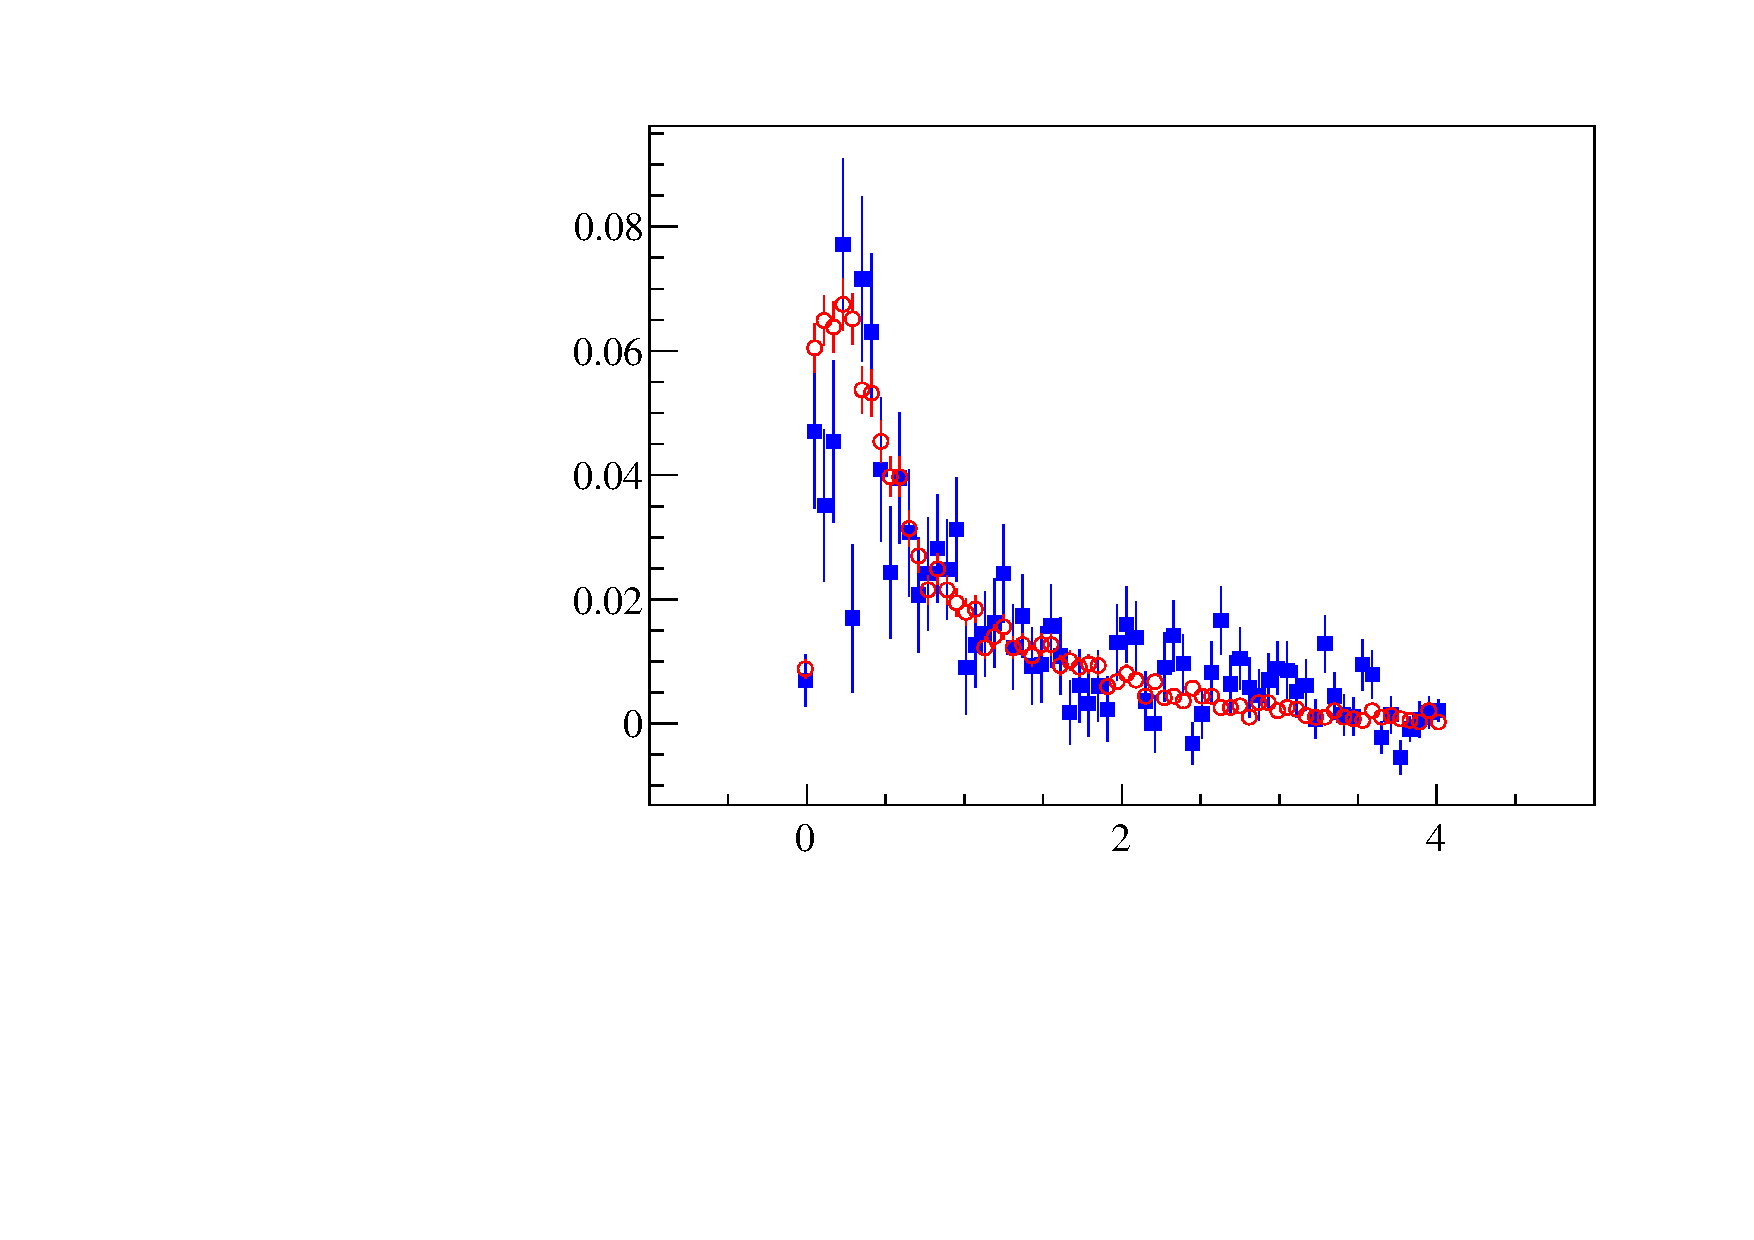
\includegraphics[width=50mm, height=35mm]{mc-data/c2_dtf_2p}
    }
    \put(100,35){
      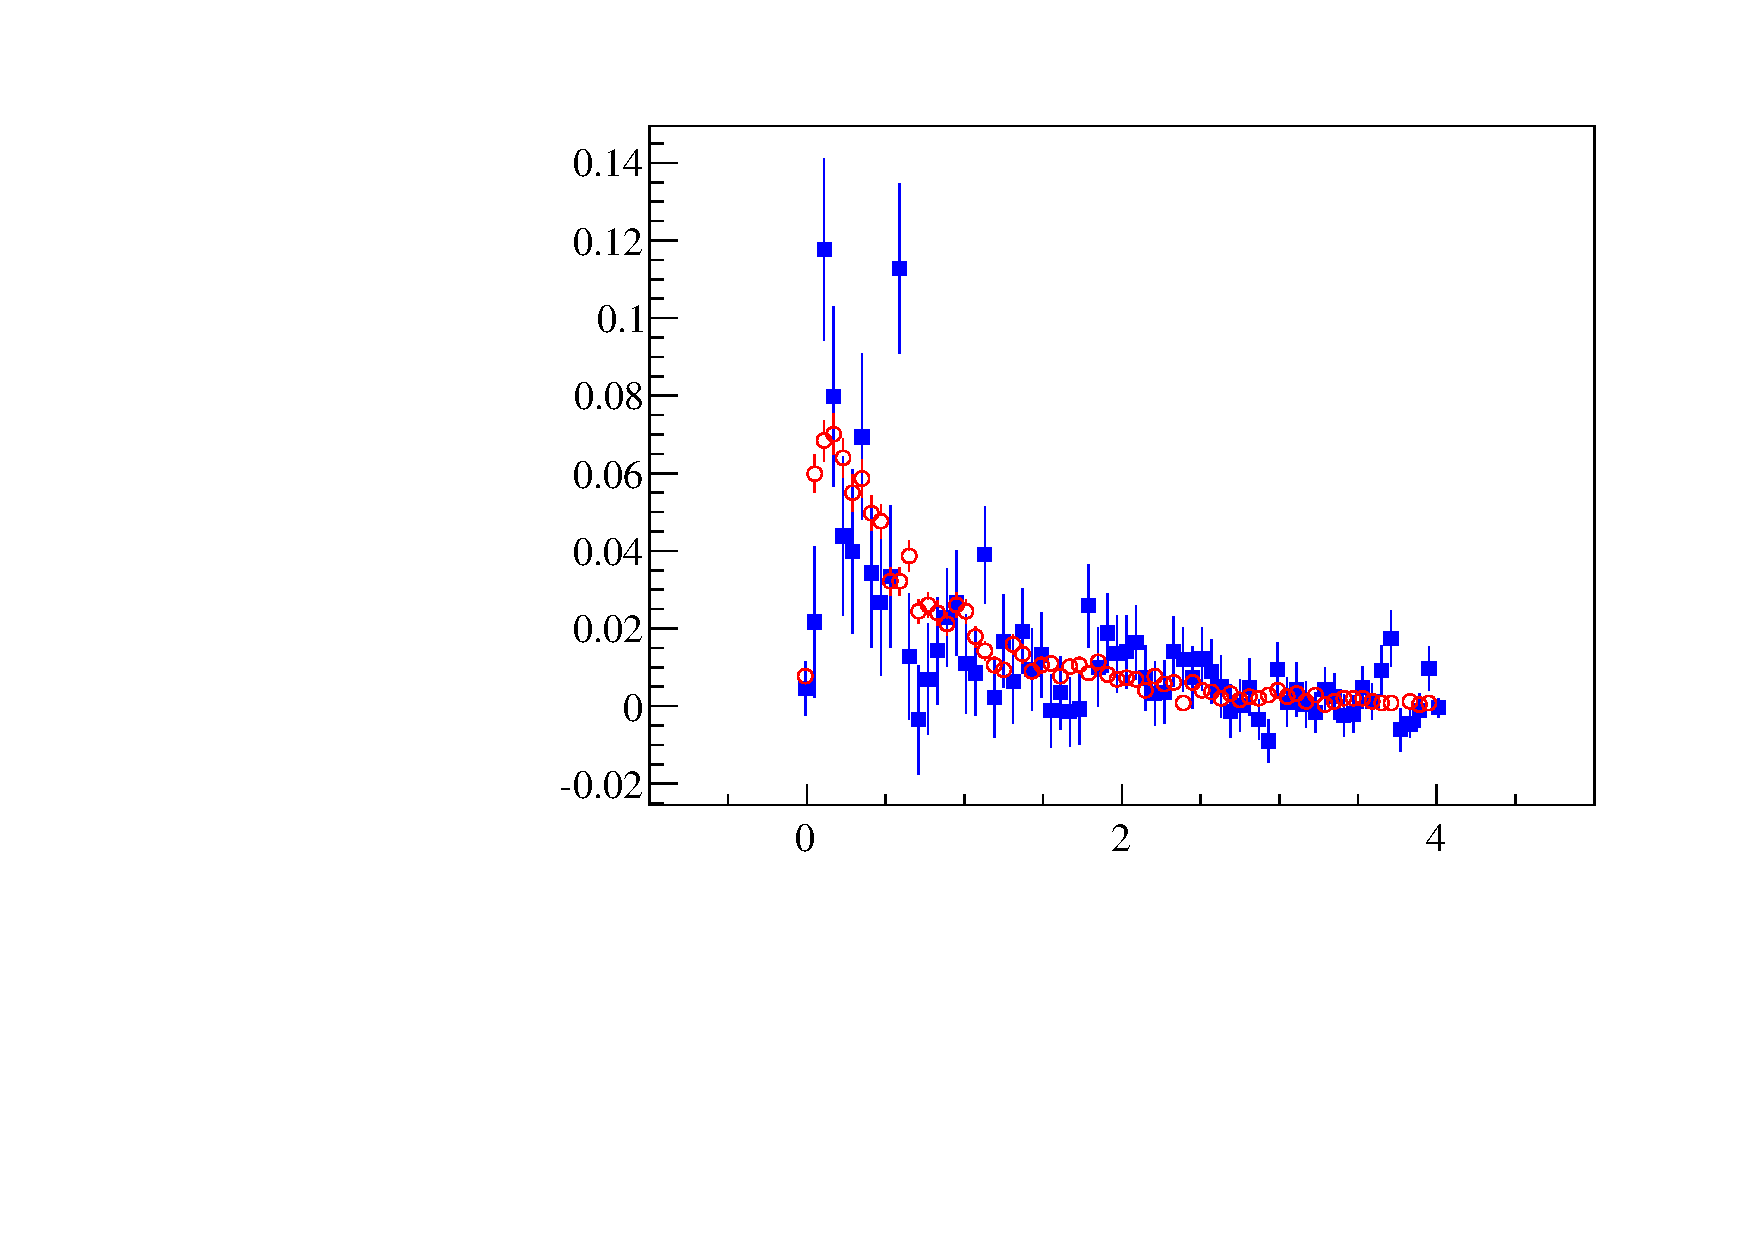
\includegraphics[width=50mm, height=35mm]{mc-data/c2_dtf_3p}
    }
    \put(0,70){
      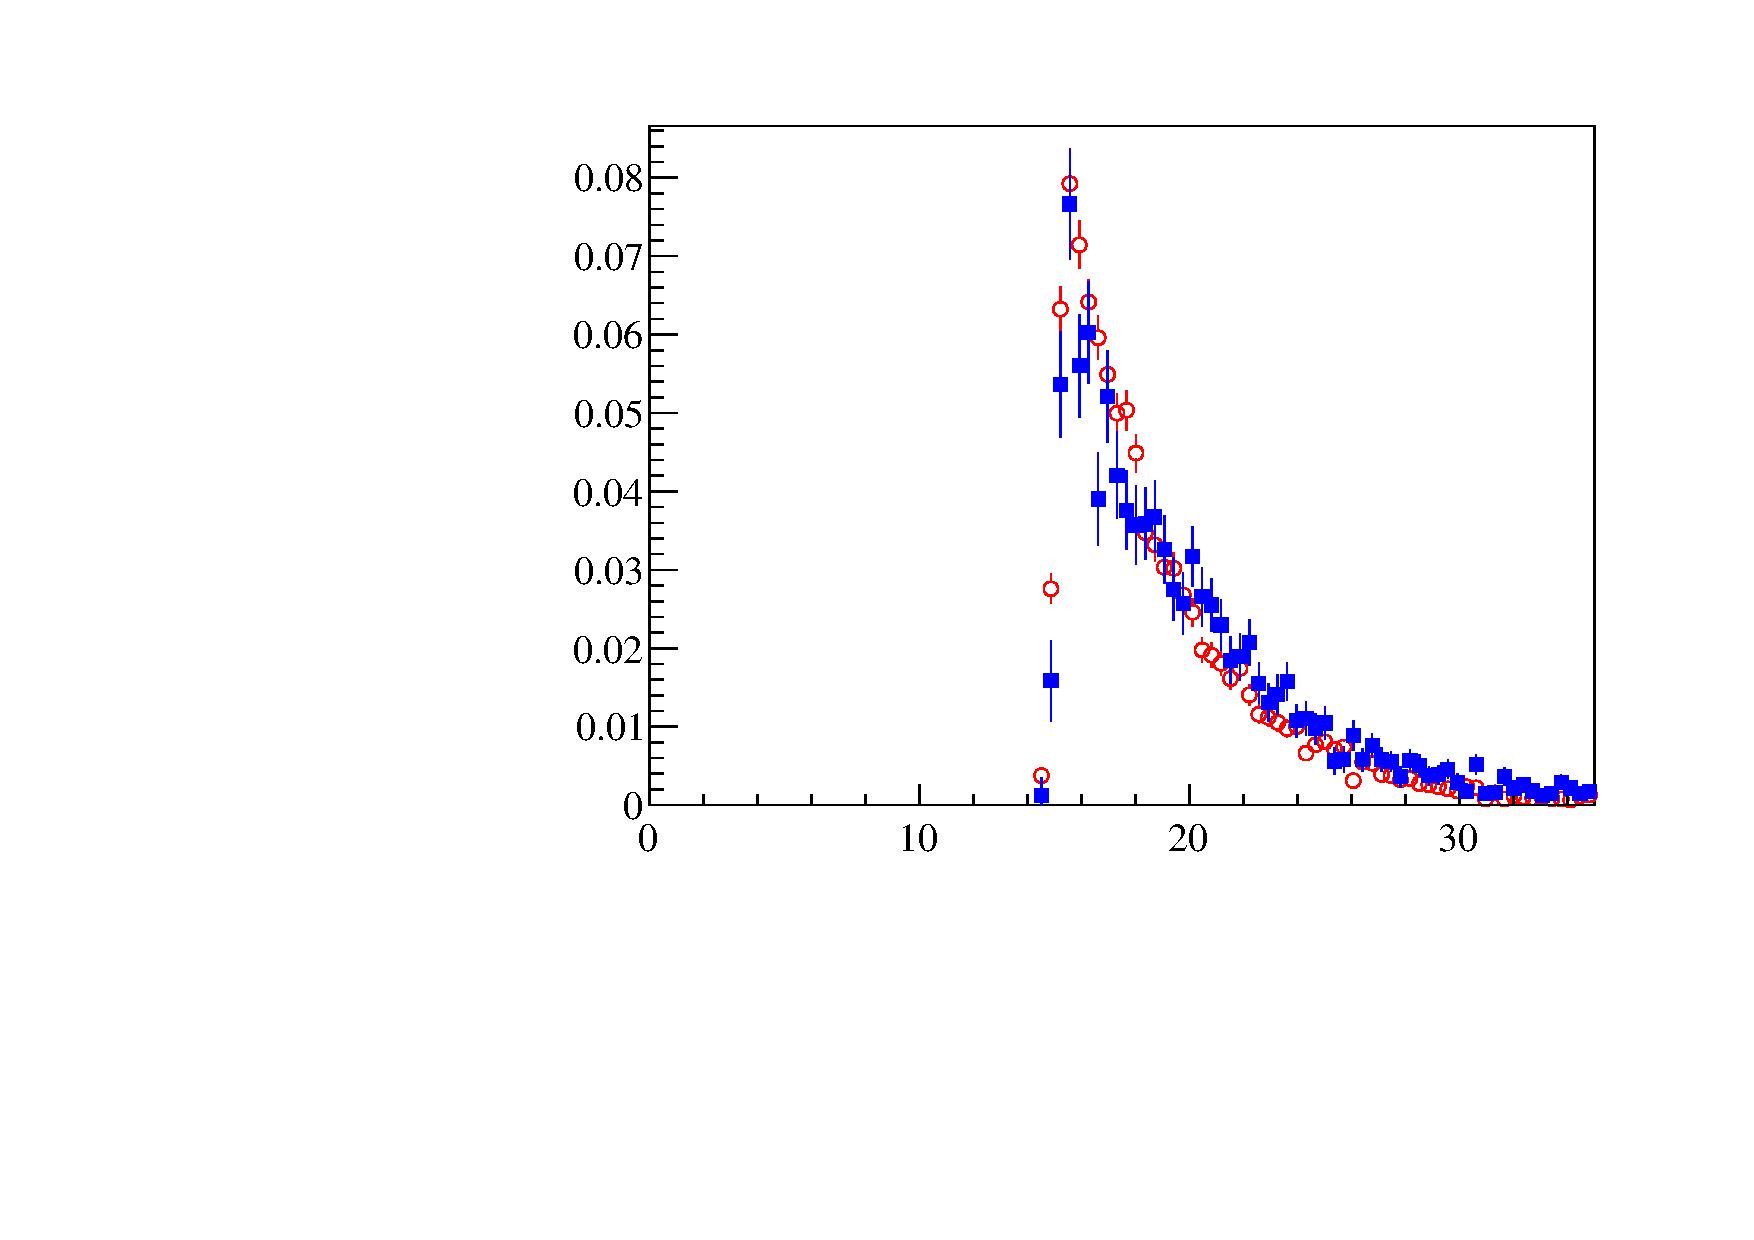
\includegraphics[width=50mm, height=35mm]{mc-data/pt_chib_1p}
    }
    \put(50,70){
      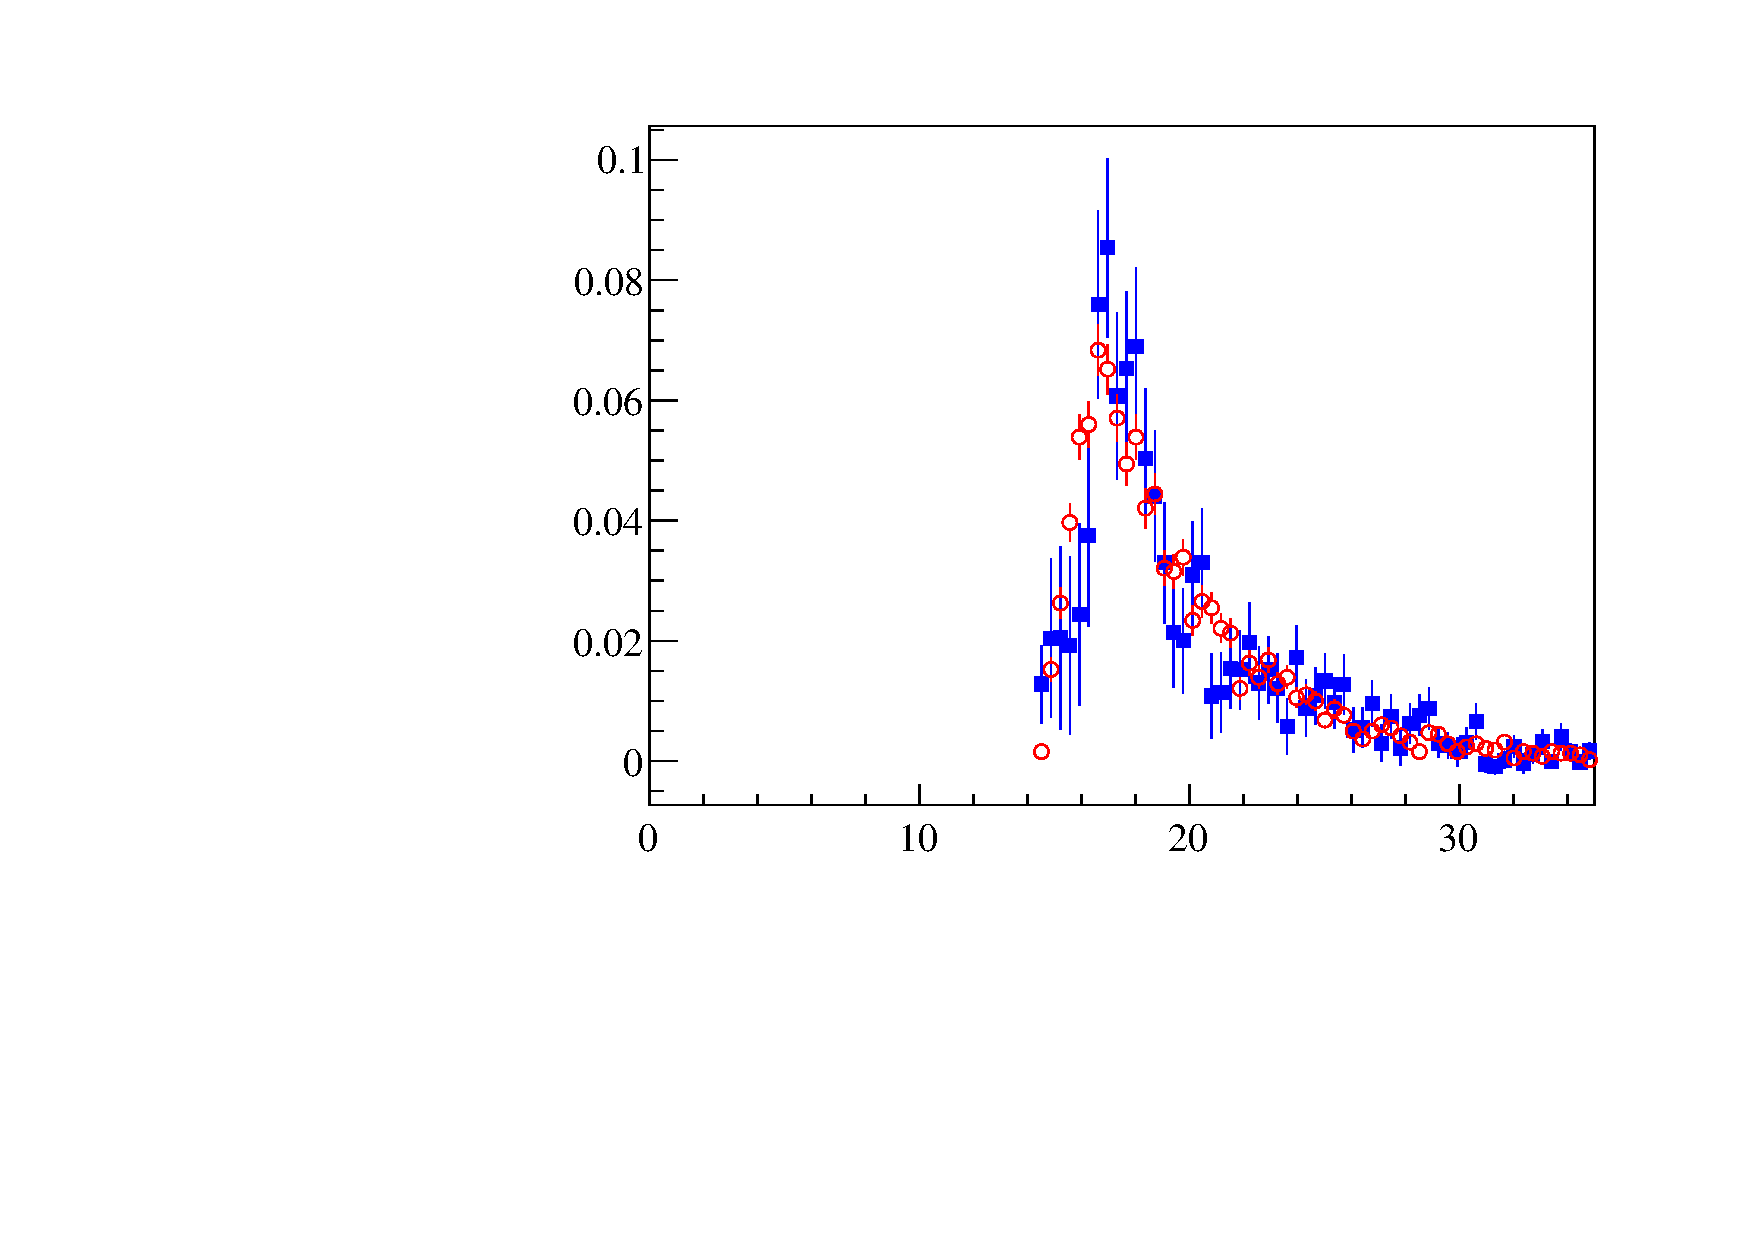
\includegraphics[width=50mm, height=35mm]{mc-data/pt_chib_2p}
    }
    \put(100,70){
      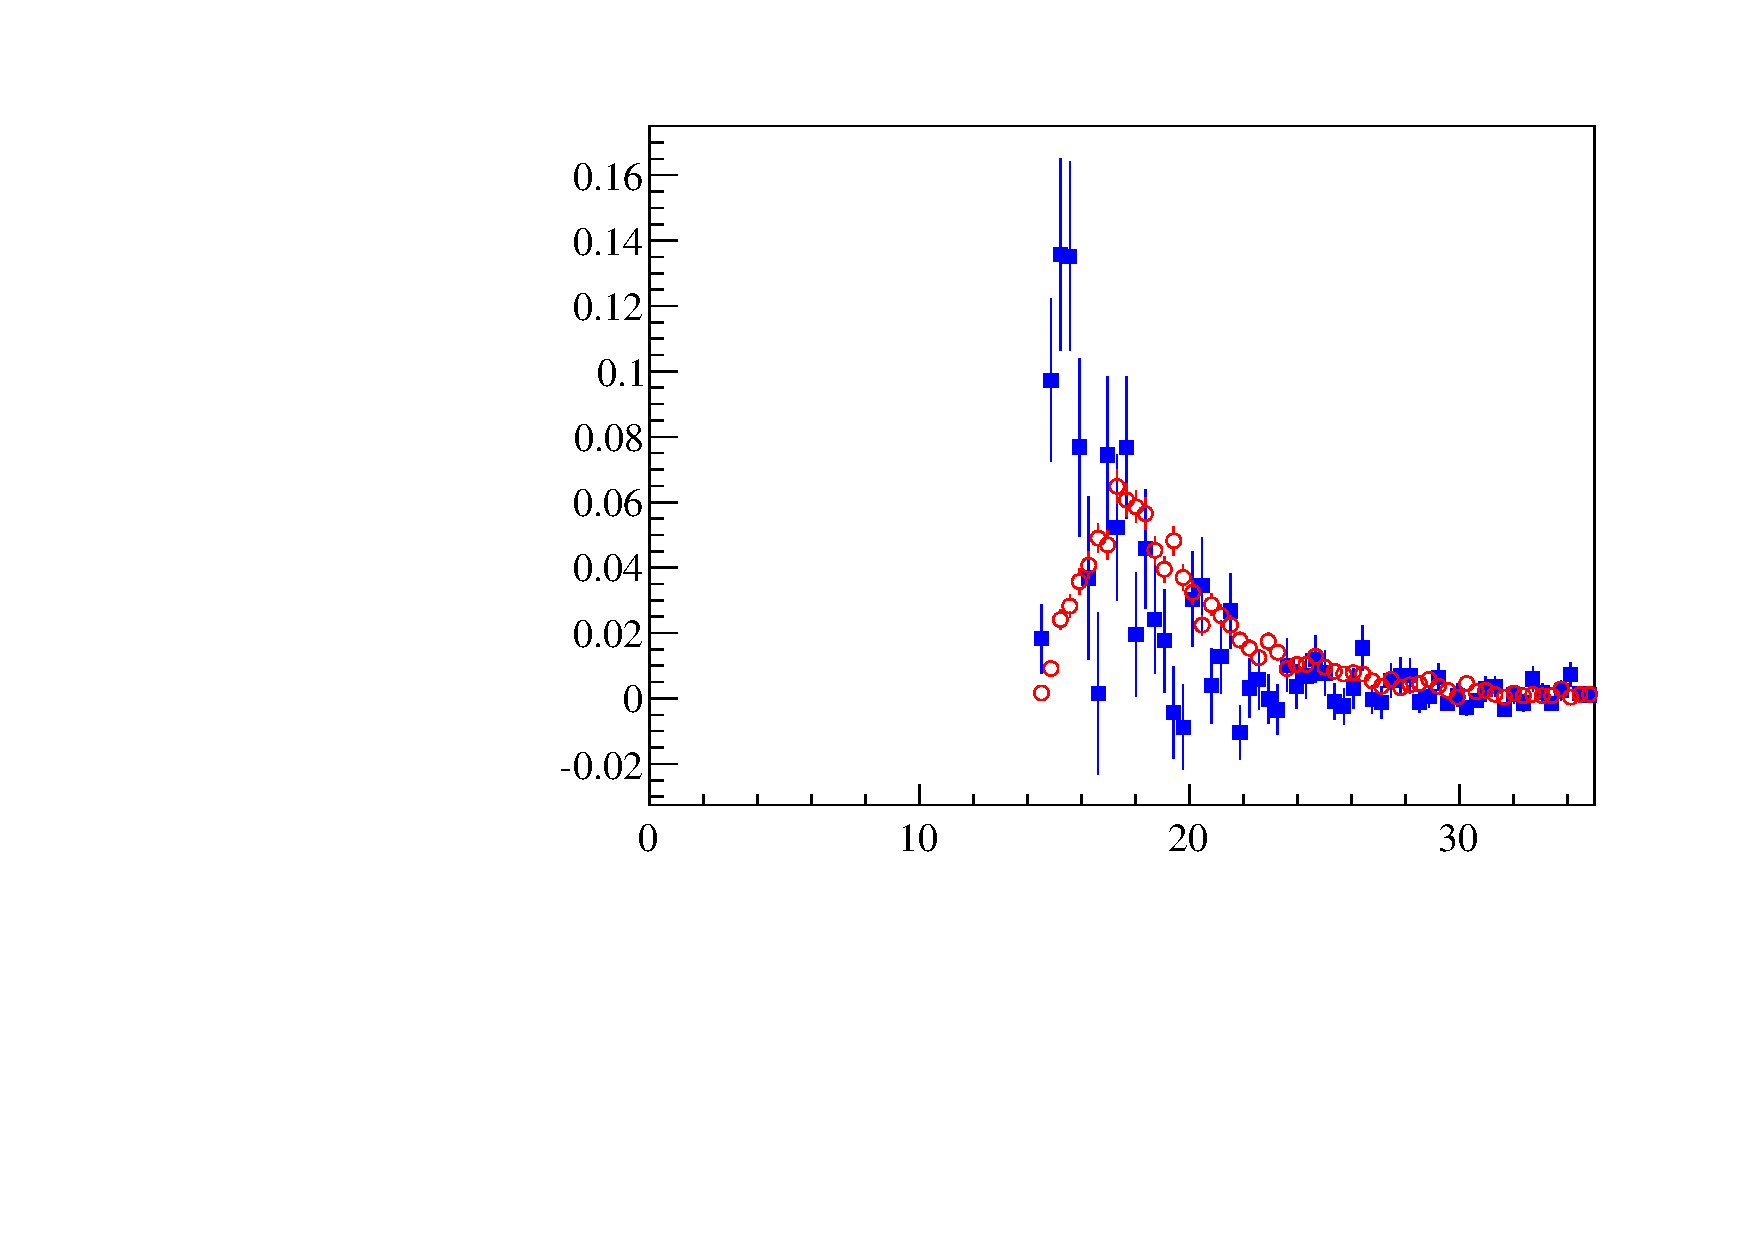
\includegraphics[width=50mm, height=35mm]{mc-data/pt_chib_3p}
    }
    \put(0,105){
      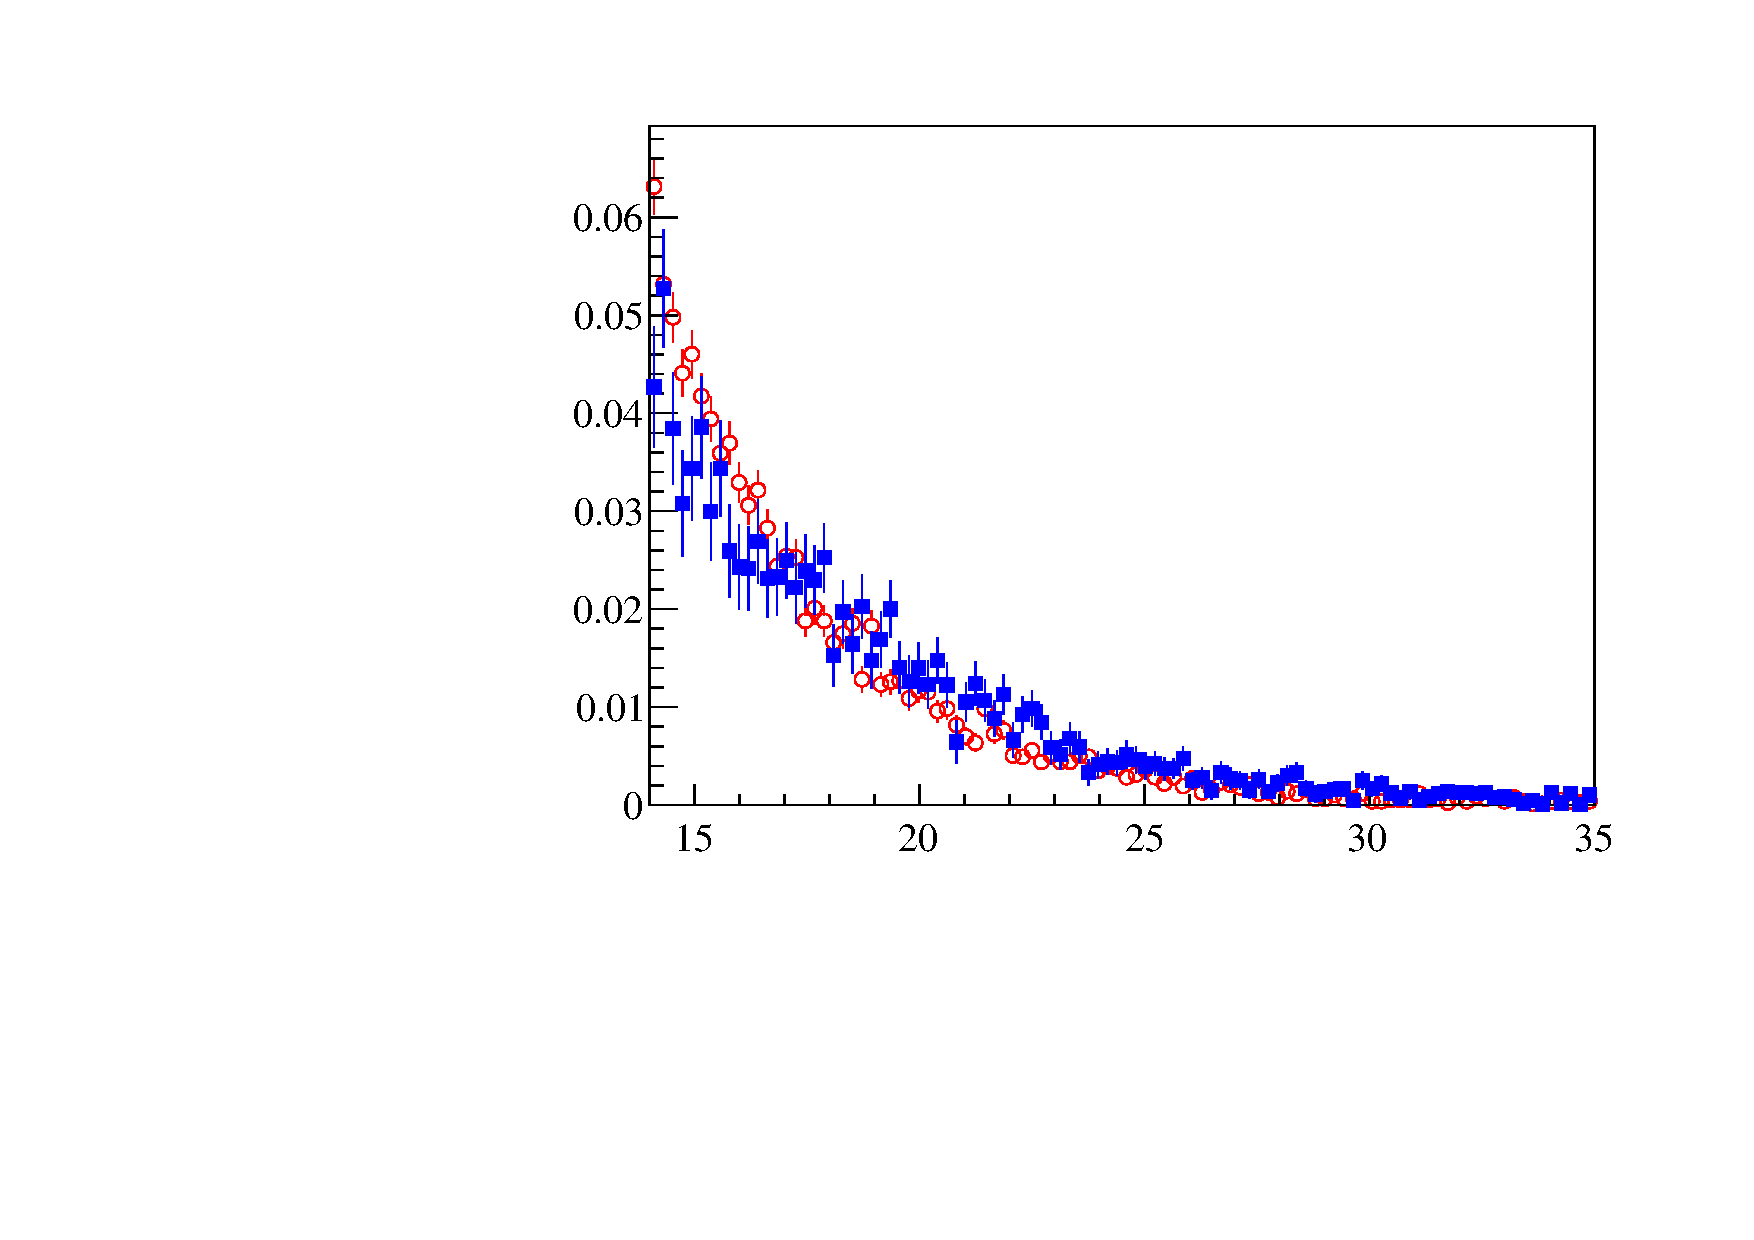
\includegraphics[width=50mm, height=35mm]{mc-data/pt_ups_1p}
    }
    \put(50,105){
      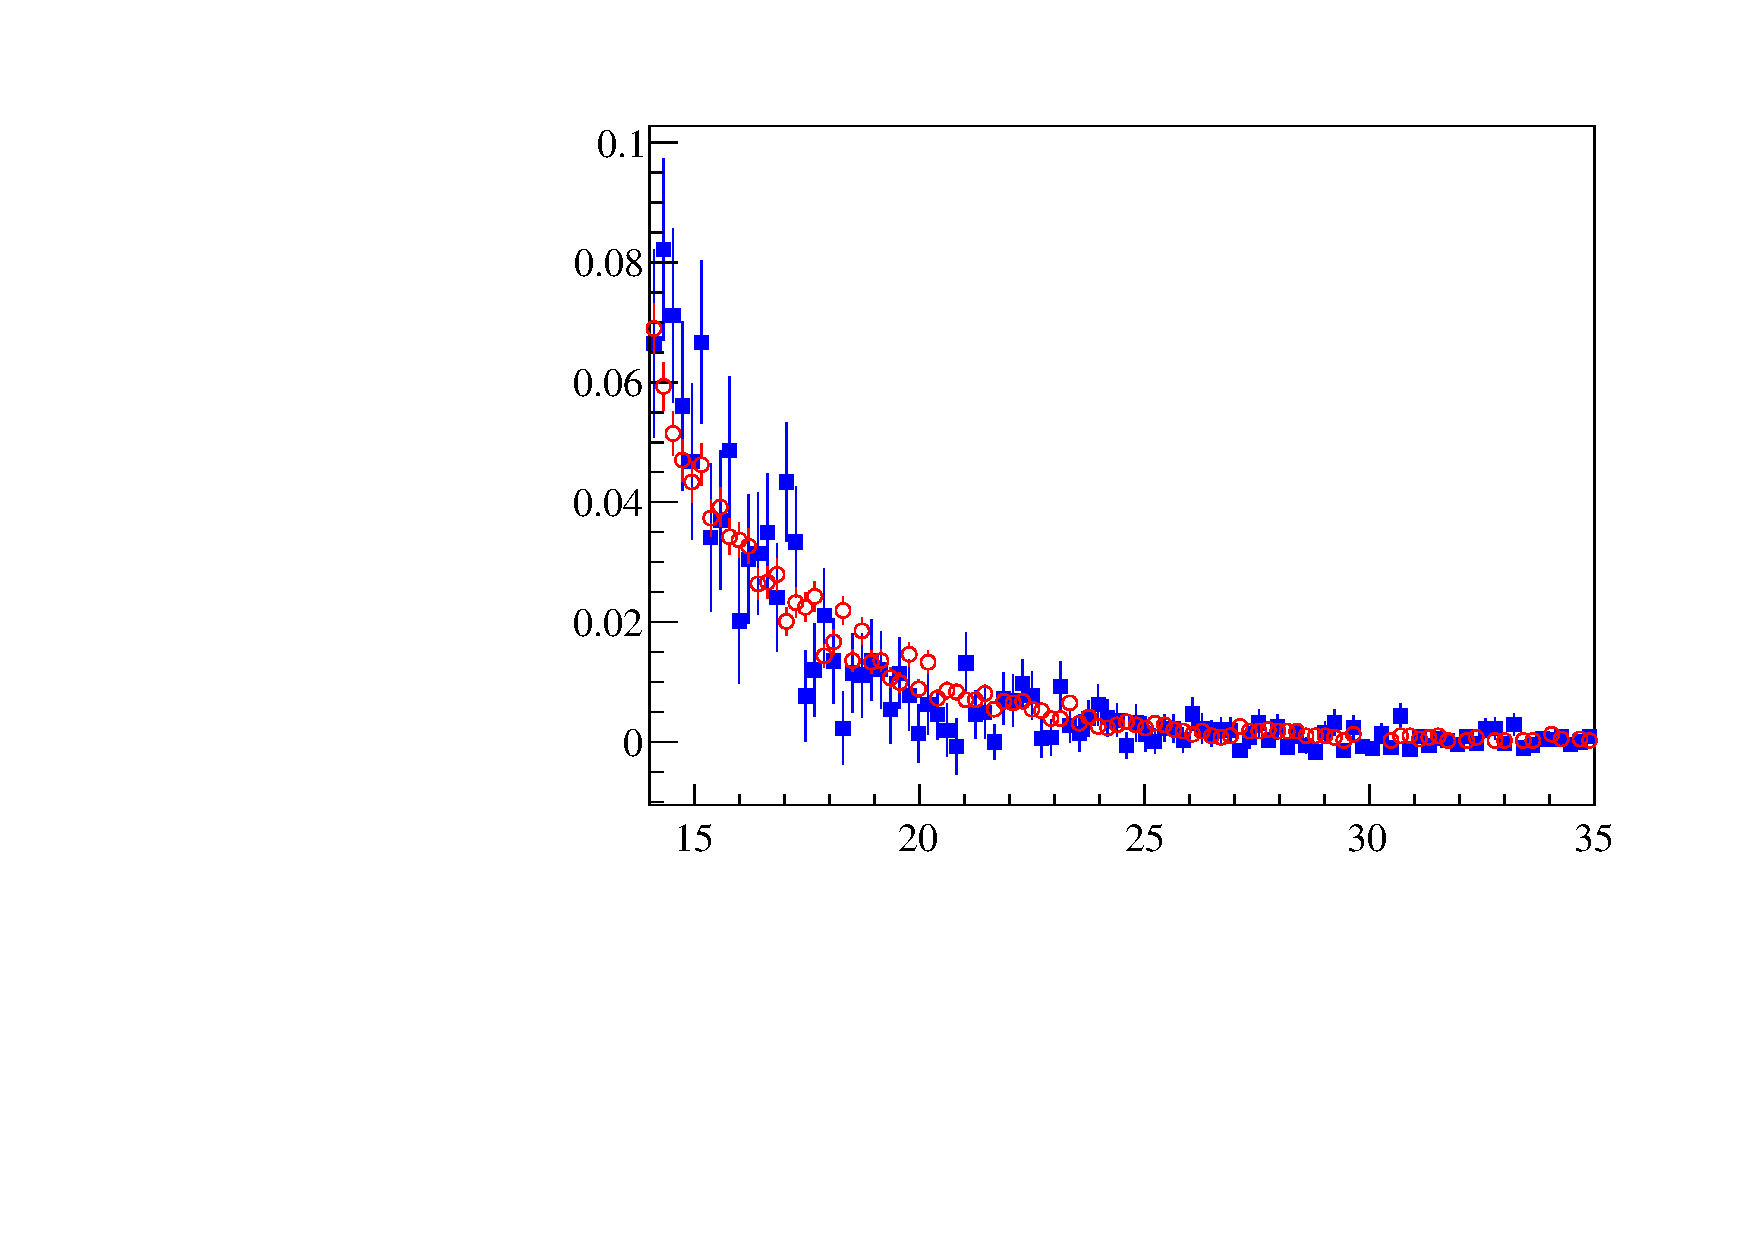
\includegraphics[width=50mm, height=35mm]{mc-data/pt_ups_2p}
    }
    \put(100,105){
      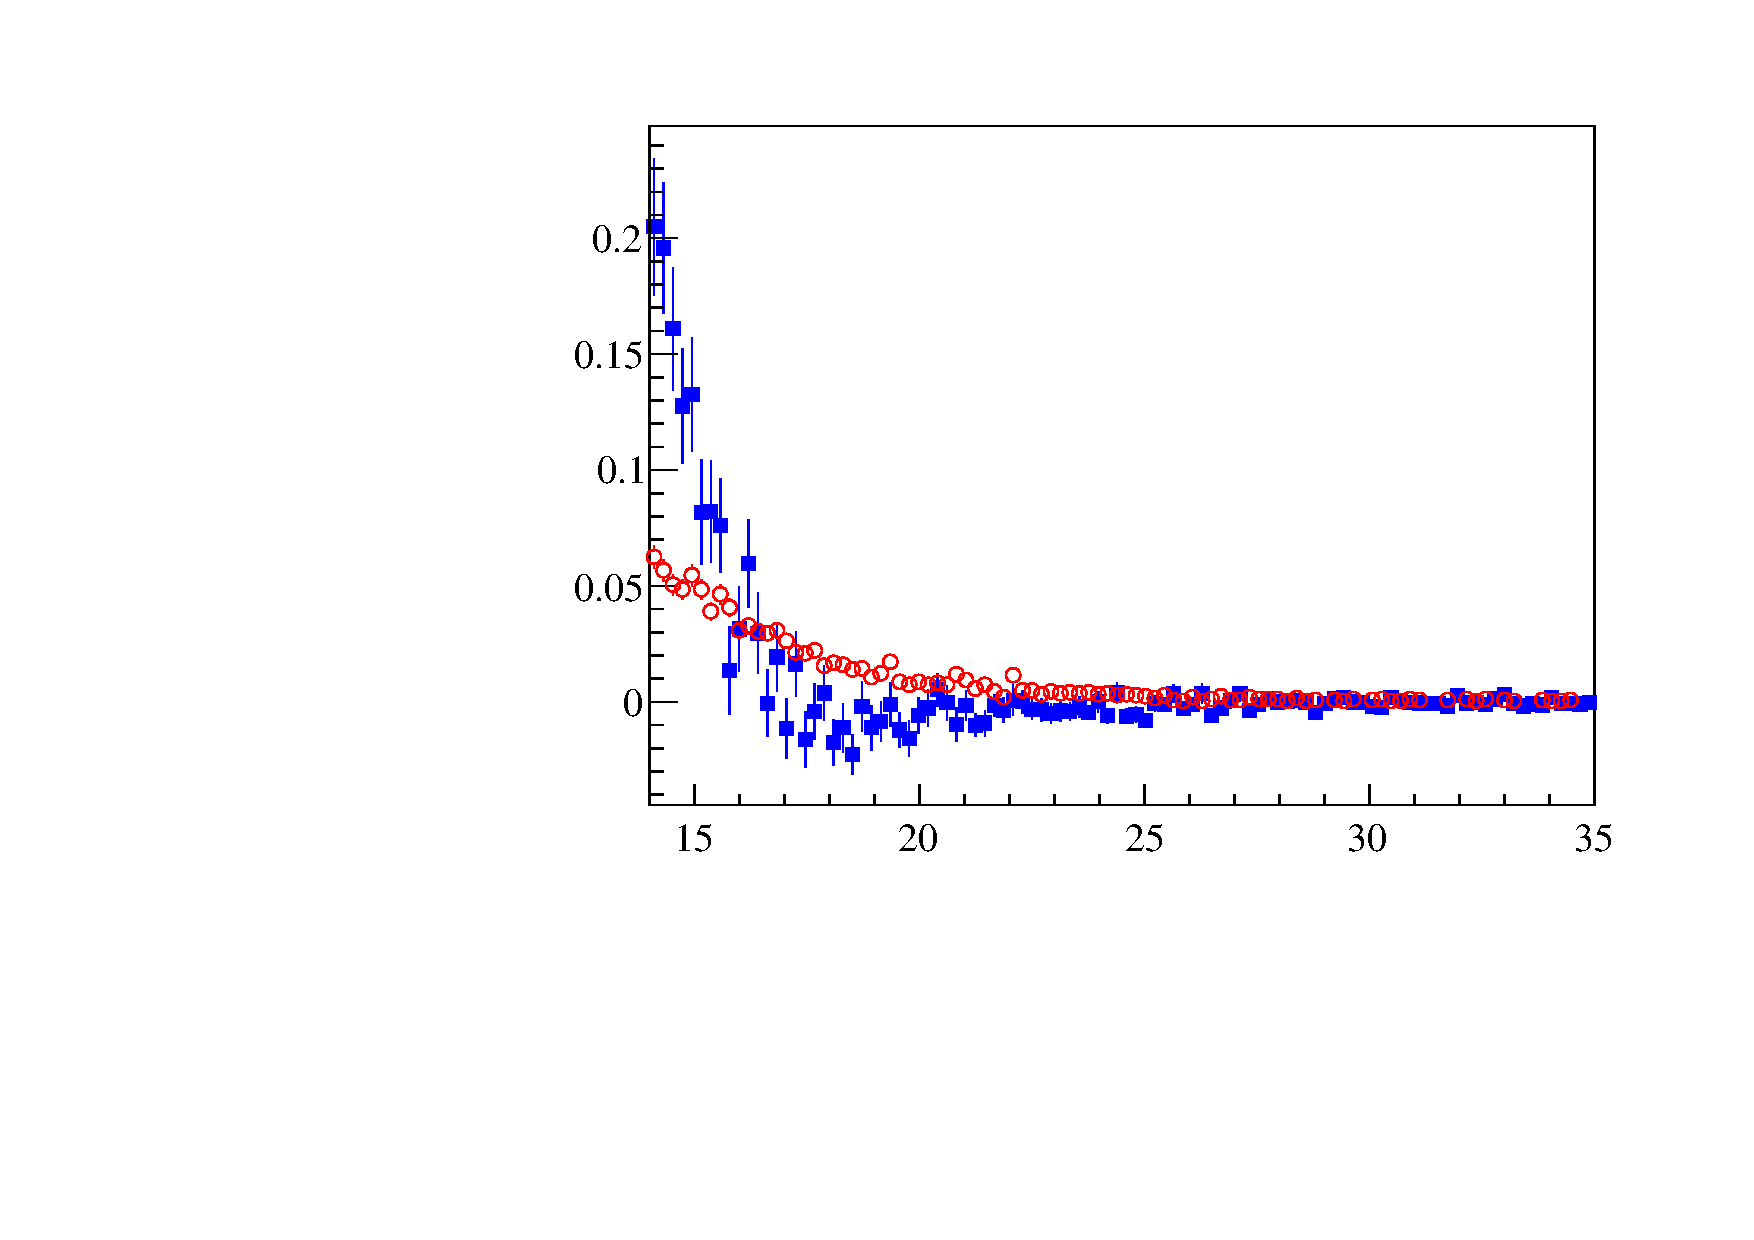
\includegraphics[width=50mm, height=35mm]{mc-data/pt_ups_3p}
    }

    \put(15,-1){\scriptsize $\gamma$ confidence level}
    \put(65,-1){\scriptsize $\gamma$ confidence level}
    \put(115,-1){\scriptsize $\gamma$ confidence level}
    \put(10,34){\scriptsize $\chisq$ of decay tree fitter}
    \put(60,34){\scriptsize $\chisq$ of decay tree fitter}
    \put(110,34){\scriptsize $\chisq$ of decay tree fitter}
    \put(20,69){\scriptsize $p_T[\chibOneP] \left[\gevcc\right]$}
    \put(70,69){\scriptsize $p_T[\chibTwoP] \left[\gevcc\right]$}
    \put(120,69){\scriptsize $p_T[\chibThreeP] \left[\gevcc\right]$}
    \put(20,104){\scriptsize $p_T[\Y1S] \left[\gevcc\right]$}
    \put(70,104){\scriptsize $p_T[\Y1S] \left[\gevcc\right]$}
    \put(120,104){\scriptsize $p_T[\Y1S] \left[\gevcc\right]$}

    \put(0,7){\scriptsize \begin{sideways}Arbitrary units\end{sideways}}
    \put(50,7){\scriptsize \begin{sideways}Arbitrary units\end{sideways}}
    \put(100,7){\scriptsize \begin{sideways}Arbitrary units\end{sideways}}
    \put(0,42){\scriptsize \begin{sideways}Arbitrary units\end{sideways}}
    \put(50,42){\scriptsize \begin{sideways}Arbitrary units\end{sideways}}
    \put(100,42){\scriptsize \begin{sideways}Arbitrary units\end{sideways}}
    \put(0,77){\scriptsize \begin{sideways}Arbitrary units\end{sideways}}
    \put(50,77){\scriptsize \begin{sideways}Arbitrary units\end{sideways}}
    \put(100,77){\scriptsize \begin{sideways}Arbitrary units\end{sideways}}
    \put(0,112){\scriptsize \begin{sideways}Arbitrary units\end{sideways}}
    \put(50,112){\scriptsize \begin{sideways}Arbitrary units\end{sideways}}
    \put(100,112){\scriptsize \begin{sideways}Arbitrary units\end{sideways}}

    \put(35,27){\scriptsize \chibOneP}
    \put(85,27){\scriptsize \chibTwoP}
    \put(135,27){\scriptsize \chibThreeP}
    \put(35,62){\scriptsize \chibOneP}
    \put(85,62){\scriptsize \chibTwoP}
    \put(135,62){\scriptsize \chibThreeP}
    \put(35,97){\scriptsize \chibOneP}
    \put(85,97){\scriptsize \chibTwoP}
    \put(135,97){\scriptsize \chibThreeP}
    \put(35,132){\scriptsize \chibOneP}
    \put(85,132){\scriptsize \chibTwoP}
    \put(135,132){\scriptsize \chibThreeP}
 
    % \graphpaper[5](0,0)(150, 175)        
  \end{picture}
}
\end{center}
\begin{block}{}
The agreement is generally very good.
\end{block}

\end{frame}
